
%A new rendering algorithm
%\begin{itemize}
%\item combines advantages of forward and backward IBR (hierarchical, multi-camera)
%\item advantages: many cameras, still very efficient
%\item Use uncertainty to maximize render quality. 
%\item Optional: good stereo rendering for depth synthesized regions (volumetric rendering)
%\end{itemize}

Our rendering algorithm consists of three stages, which are closely coupled:
appearance selection (or camera/view selection), 
appearance mapping (warp/backprojection) and appearance synthesis (blending). 
An important requirement throughout this process is the preservation 
of depth contours and depth relationships in the scene.
%In all these steps, the IBR algorithm should preser contours-depth relationships.
Appearance selection and mapping can be defined at the level of rays, pixels,
local regions or even higher level segments. 
As \cite{Zitnick:2004:viewinterp} demostrated, choosing regions represented by superpixels provides robustness to uncertainty
(of several aspects of the image formation process and calibration
offsets).

Rendering algorithms with forward mapping do not enforce the 
\textbf{\emph{continuity}}
property of the novel view \cite{ULR}, since they 
result in popping and produce incomplete regions when the subset
of selected cameras changes.
%producing jumps and
%in-completions when the subset of selected cameras changes. 
To favor speed, forward algorithms select cameras based on spatial proximity with no warranty
of coverage. 
%Popping, spatial discontinuities and incompleteness are common artifacts found in these methods. 
On the other hand, backprojection methods %need an invertible transformation
%or they 
rely completely on the reconstructed geometry to look up source appearance
for the novel view or require some form of dense correspondence~\cite{dibr}. 
The novel view is completed continuously, but only in 
regions where some geometry or correspondences with input images exists. \TODO{mnention that color is interpolated?}. 

In our unified algorithm new views are synthesized by first using 
backprojection for appearance selection at the level of local regions, 
then using forward warping for appearance mapping and finally
blending based on our uncertainty model.
%We formulate the problem of render a novel view as a backward search
%(appearance selection) for a forward mapping (appearance mapping)
%followed for a blending counting for uncertainty (appearance synthesis). 

\begin{figure}[t]
	%\vspace{0.1in}
	\centering
	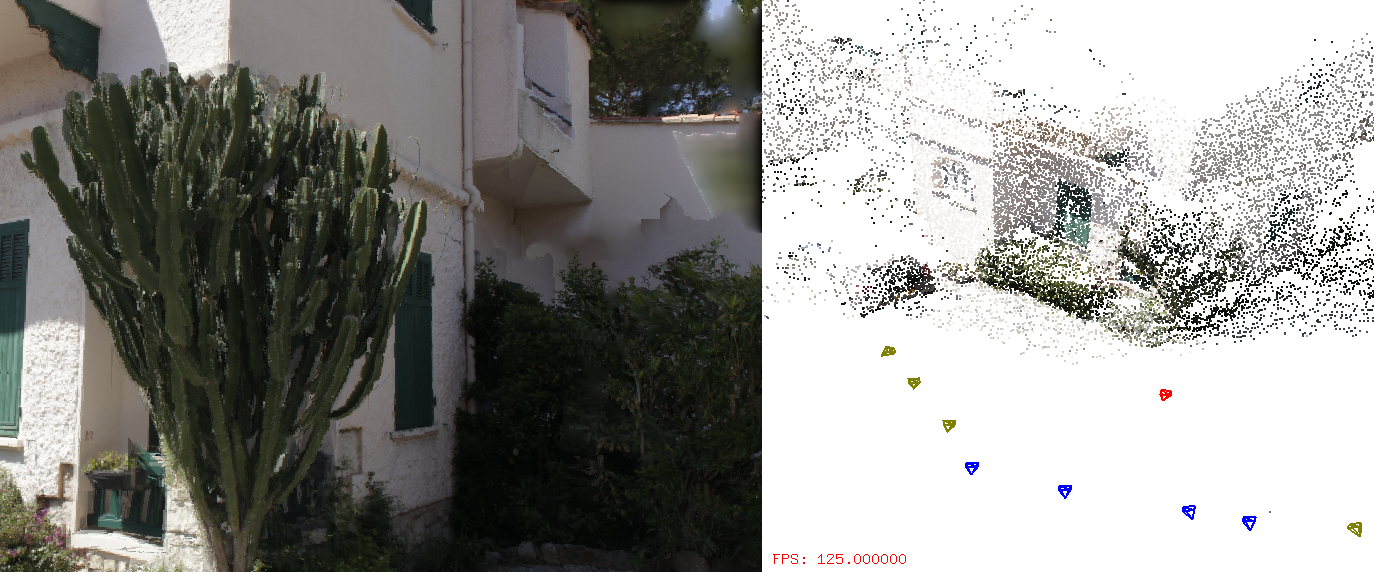
\includegraphics[scale=0.22]{graphics/cam_selection_problem_1.png}
	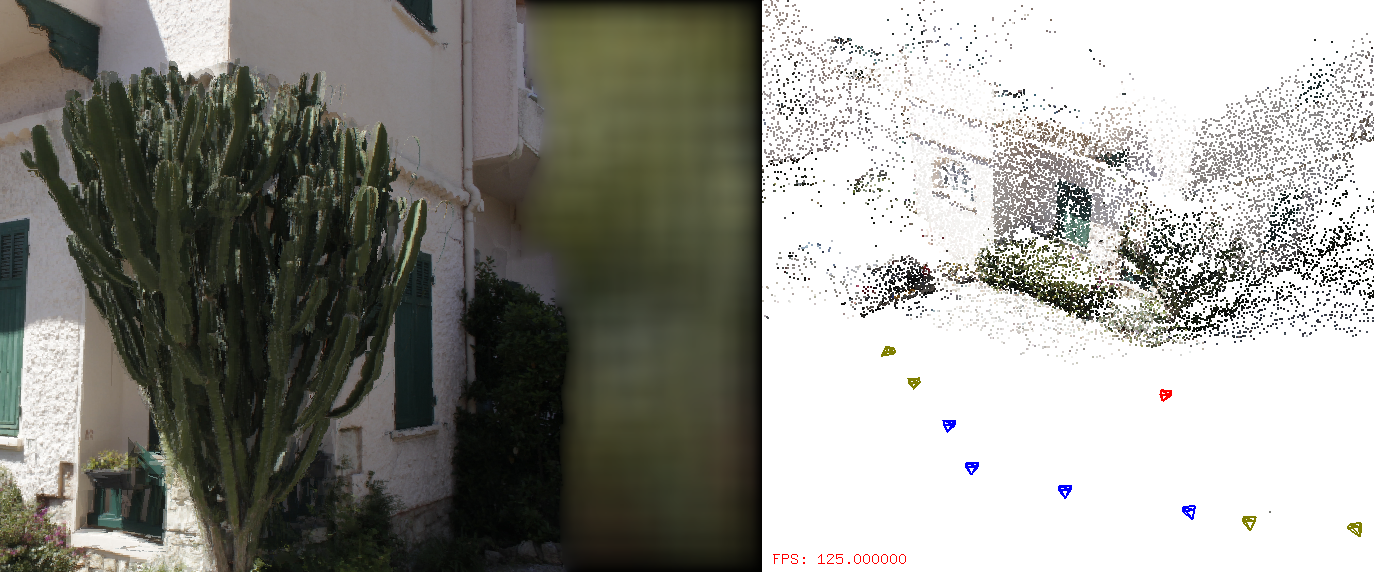
\includegraphics[scale=0.22]{graphics/cam_selection_problem_2.png}	
	\caption{\label{fig:cam_select_problem} 
		Camera selection problem of forward mapping: On the right, we show the input viewpoints (in green), the selected viewpoints (in blue) and the novel viewpoint. Upper row: a novel image generated from the point of view in red. Lower row: the view point has changed one unit w.r.t. the upper row. A discontinuity apprears on the right of the image.}
\end{figure}


\subsection{Appearance Selection:}

%The backward search tries 
We first find regions $S^{i}$ of input camera $C_{i}$
to be used in a further forward mapping and synthesis of a novel view,
using backprojection.
Each region is denoted with $s_{j}^{i}$, where $S^{i}=\{s_{j}^{i}\}$.
Process:
\begin{enumerate}
	\item Overlay a regular grid on the viewport of the novel camera. Cells of the grid are spaced $m$ pixels.
	\item Render a depth map and uncertainty on the novel view.
	\item The depth and uncertainty associated to each vertex of the grid are
	used to look up $s_{j}^{i}$ in each $C_{i}$. The bigger the uncertainty,
	the more chances to hit more than one superpixel $s_{j}^{i}$ in
	$C_{i}$ \TODO{()can be also a function of the contour of superpixel)}.
	\item Create $S^{i}$ as $\cup_j s_{j}^{i}$ in $C_{i}$ assigned to vertices of the grid.
\end{enumerate}
%The expected number of pixels inside of a superpixels is $n^{2}$
%where: $n^{2}=width*height/number\_superpixels$ (see fig). Then $m=(1-\alpha)*n^{2}$,
%where $\alpha$ is the expected overlapping percentage of the transformed superpixels.

\begin{figure}[t]
	%\vspace{0.1in}
	\centering
	
\includegraphics[scale=0.25]{graphics/spixels_overlap.png}
	\caption{\label{fig:spixel_overlaping} 
	In red, the expected overlaping $\alpha$ of mapped superpixels.}
\end{figure}

The expected number of pixels inside a superpixel is $n^{2}$
where: $n^{2}=w \times h/n_s$ (see fig) where the images has resolution
$w \times h$ and $n_s$ is the number of superpixels. Then $m=(1-\alpha)*n^{2}$,
where $\alpha$ is the expected overlapping percentage of the transformed superpixels.

\subsection{Appearance Mapping}

The list of superpixels collected by the appearance selection step
is forward warped as in ~\cite{ODD15}, using the selected 
rendering algorithm. Since the expected number of superpixels is small,
this approach combines the advantages of backprojection methods,
i.e., using a larger number of cameras and those of oversegmentation-based forward warping approaches, i.e., preservation of depth boundaries and efficient projection (since the total number of superpixels is low).
%to an apparent correct place!


\subsection{Appearance Synthesis (Blending and filtering)}

Our synthesis approach will use our uncertainty model to
achieve the best possible quality.
Uncertainty can be used to determine how many images to blend
(typically one or two), and the corresponding weights to be used.
